Image fusion is a process that merges several images, possibly acquired in diverse conditions or with different cameras, into one image with higher quality, more details and consequently more useful for humans and computer tasks \cite{mitchell2010image}. Examples of image fusion applications are noise reduction, edge enhancement and super-resolution. One prominent use of image fusion occurs in medical imaging fields; the quality of information about illnesses, cells, clinical analysis and several other medical tasks (including the computer-assisted ones) have found profitable results from the image fusion techniques and led themselves to better and faster decisions when it comes to human beings \cite{james2014medical}. There are also relevant applications in remote sensing multispectral images, segmentation of regions in different colourspaces, biometry: the pan-sharpening process is the generation of an high resolution multispectral image from low to high resolution ones, K-Means segmentation and fusion of pixels in the RGB and the Iris Recognition biometric process with video frames are examples of such tasks, respectively \cite{mitchell2010image}.

\subsection{General Framework}

Still according to \citeonline{mitchell2010image}, the general framework for the image fusion procedure consists of four stages: \emph{Multiple Input Images}, \emph{Common Representational Format}, \emph{Fusion} and \emph{Display}.
The multiple input images stage is simply the acquisition of the images to be merged. There are several approaches to this: the dataset may be captured from different sensors, on distinct light conditions or angles, with different magnifications, on several focus settings and with temporal measurements if the scene changes through time.

If the acquired dataset images do not share the same features such as dimension, rotation angle and resolution, then the images should be pre-processed in order to achieve a common state. This configures the common representational format step, which generates a new and temporary dataset with the same properties, e.g. color space, dimensions, and noise level. The fusion stage employs a decision method in order to dictate which regions, objects, colors or details will compose the final image; there are some methods that rely on the wavelet transform, for example. Finally, the display stage provides a view for the resulting image, which can be used directly for any further task or even be the input for other image processing operation. Figure \ref{fig:fusion_general_framework} depicts an arbitrary example of the four stages:

\begin{figure}[H]
	\centering
	\caption{\label{fig:fusion_general_framework}Image fusion general framework. (a) Multiple Input Images, (b) Common Representational Format, (c) Fusion and (d) Display.}
	\begin{center}
    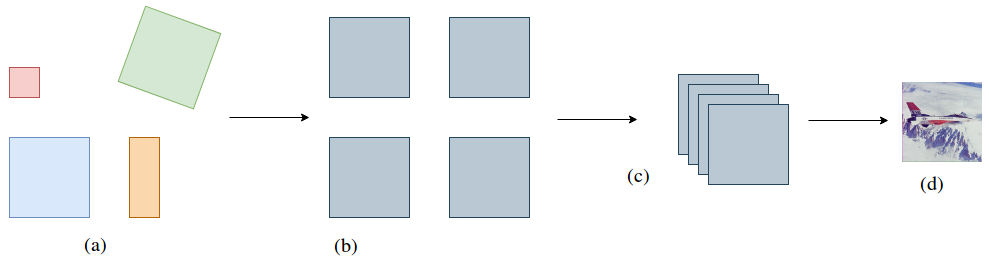
\includegraphics[scale=0.4]{images/image_fusion_scheme.png}
	\end{center}
	\centering
    \fautor
\end{figure}

The four arbitrary images in Figure~\ref{fig:fusion_general_framework}.\textbf{(a)} represents different images of the same scene, taken at different resolutions, rotation angles and shapes. In Figure~\ref{fig:fusion_general_framework}.\textbf{(b)}, the images are all reshaped, converted to a common color space and ready to undergo the processing algorithm which will transform them into feature vectors. Figure~\ref{fig:fusion_general_framework}.\textbf{(c)} represents the image fusion by means of an arbitrary fusion rule. The resulting image is depicted in Figure~\ref{fig:fusion_general_framework}.\textbf{(d)}. Since image fusion is only one branch of data fusion field, this procedure has a wide variety approaches and methods; hence, the domain will be restricted to the multifocus image fusion and some relevant related work will be presented in Chapter~\ref{chapter:related-work}.